\section{Results}

\subsection{Estimating traits via PROSPECT inversion}

\begin{figure}
  \centering
  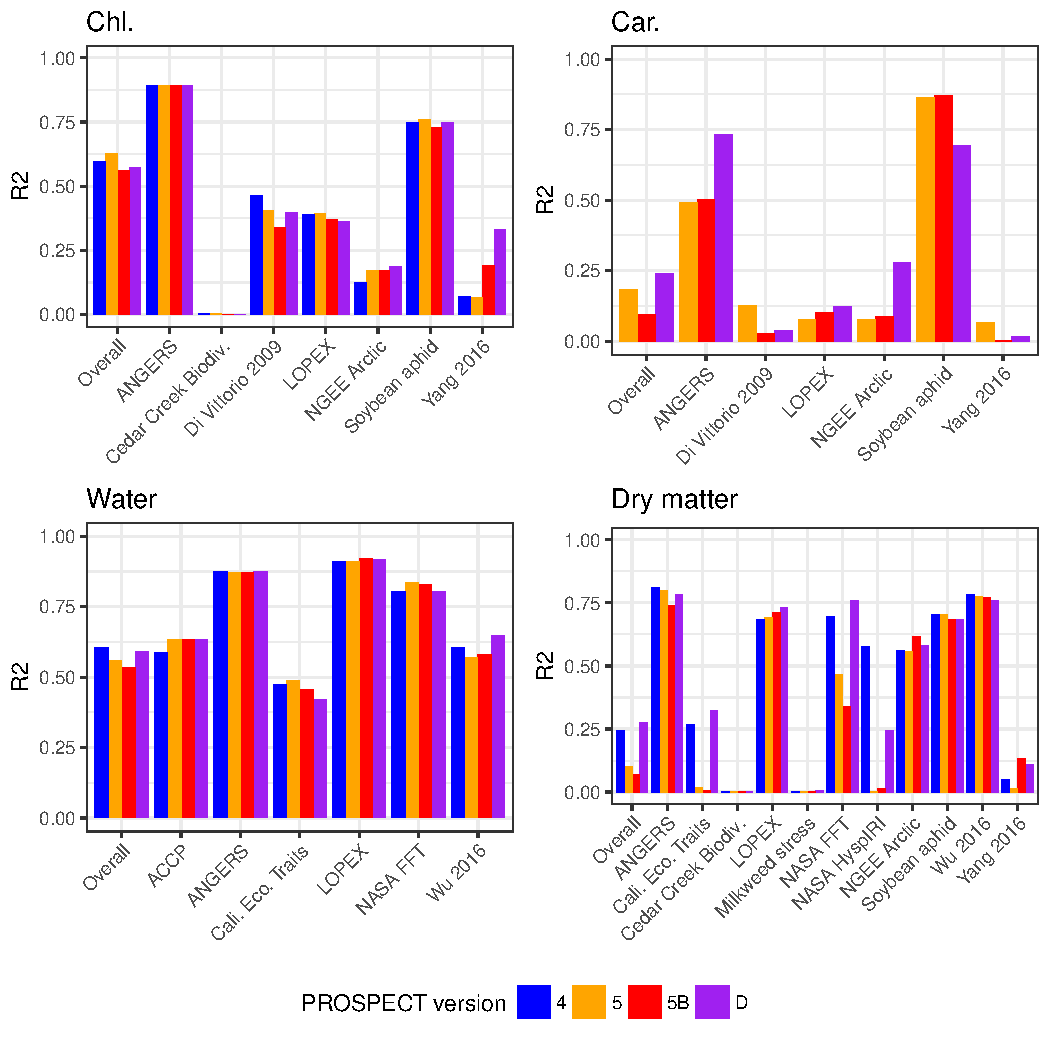
\includegraphics[width=\textwidth]{{figures/project_validation_summary}.pdf}
  \caption{\
    Validation of PROSPECT against observed trait values, by project and PROSPECT version.
    Y-axis represents $R^2$ values for robust linear regression.
  }\label{fig:project_validation_summary}
\end{figure}

Across most projects and traits, the four different PROSPECT versions performed similarly in terms of their ability to retrieve traits (Figure~\ref{fig:project_validation_summary}).
For all versions of PROSPECT, leaf water content was consistently the most accurate trait retrieved, while retrievals of other traits were highly project-specific.
For several projects spanning a large range of species (Cali.\ Eco.\ Traits, NASA FFT, and NASA HyspIRI), moving from chlorophyll as the only pigment (PROSPECT 4) to chlorophyll and carotenoids (PROSPECT 5/5B) drastically reduced inversion accuracy of dry matter contents, but this accuracy was restored by the further addition of anthocyanins and modification of the refractive index in PROSPECT D (Figure~\ref{fig:project_validation_summary}).
Because PROSPECT-D also retrieves anthocyanin content and generally performed as well or better than other versions, it was the version selected for subsequent analyses.

\begin{figure}
  \centering
  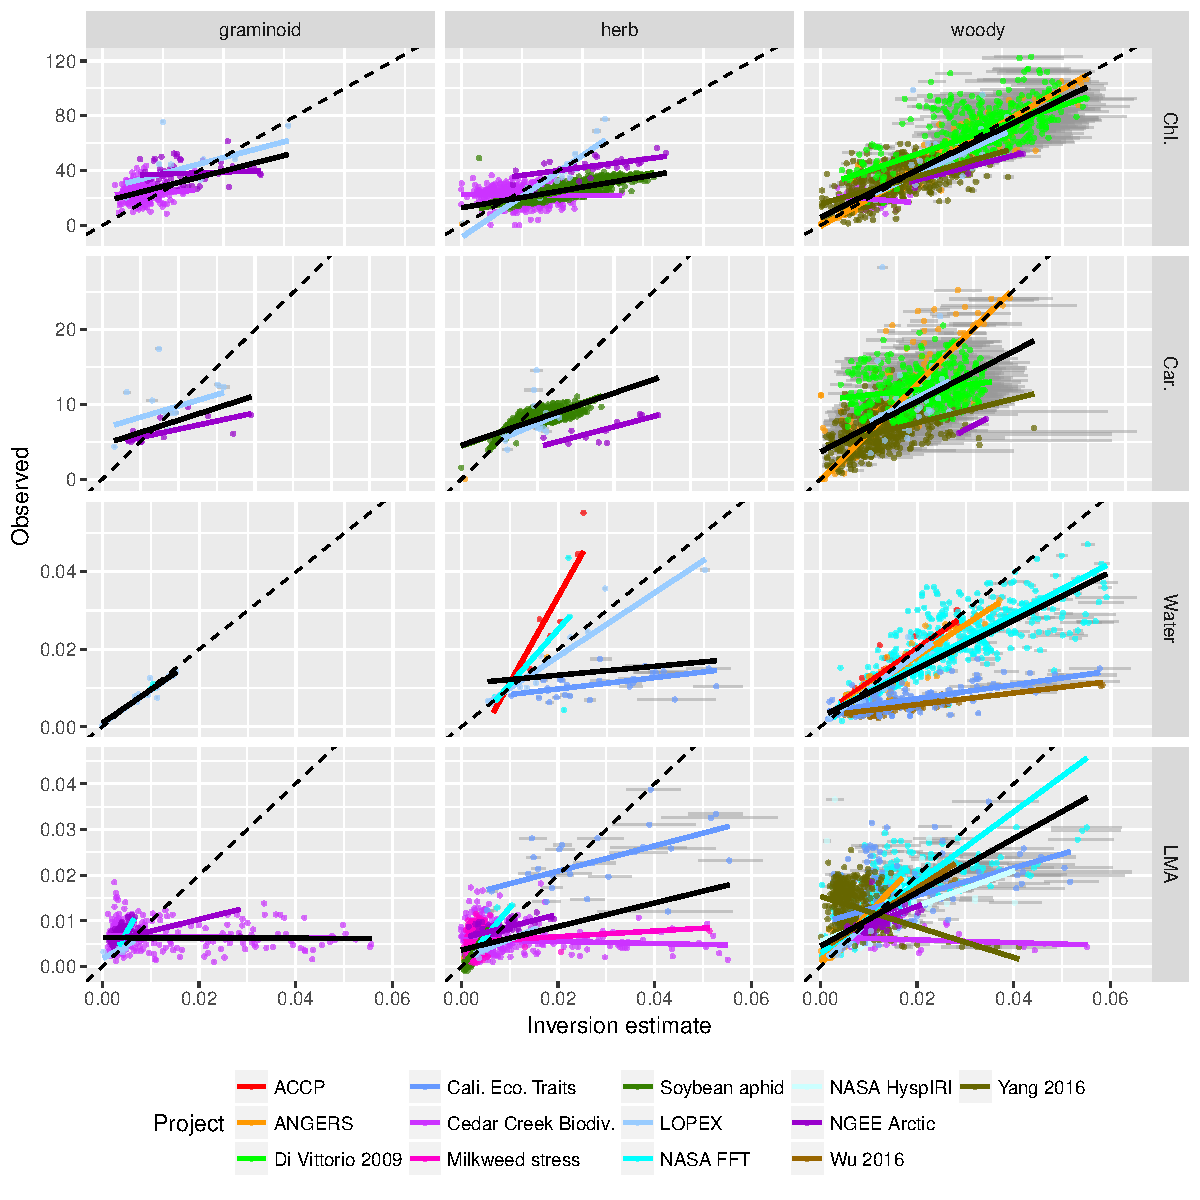
\includegraphics[width=\textwidth]{3_prospect/figures/validation_by_gf.pdf}
  \caption{\
    Validation of PROSPECT-D against observed trait values.
    Grey lines indicate 95\% confidence intervals around trait estimates.
    Solid, colored lines are robust regressions fit to the data by project and functional type.
    The solid black line is a regression fit to all of the data for a given functional type.
    The dashed black line is a 1 to 1 fit.
  }\label{fig:prospect_D_validation}
\end{figure}

\begin{figure}
  \centering
  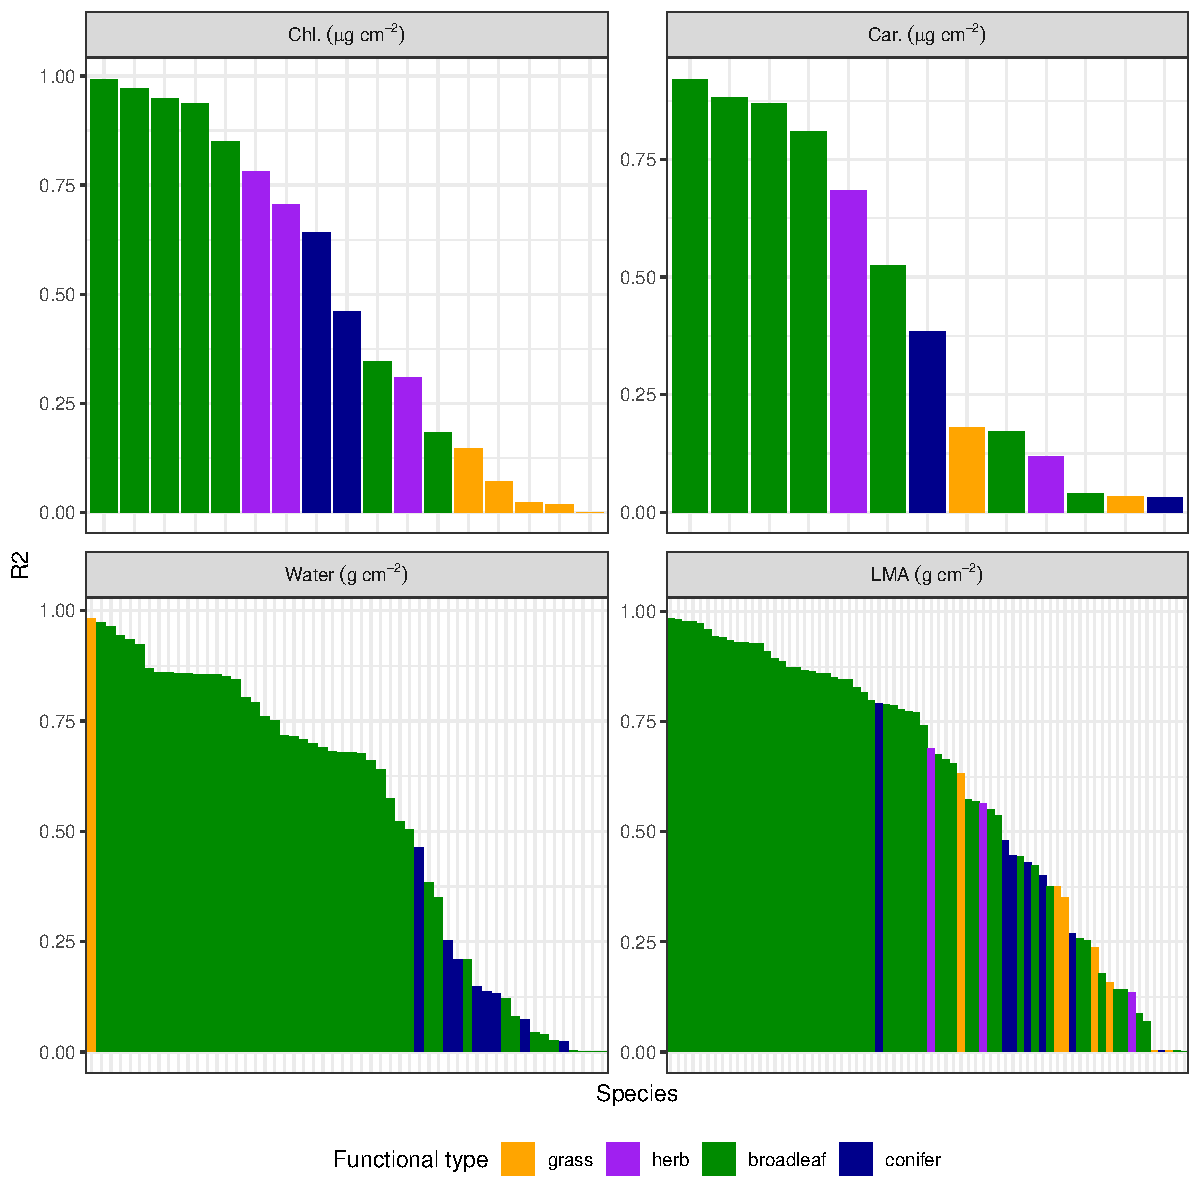
\includegraphics[width=\textwidth]{3_prospect/figures/r2_by_gf.pdf}
  \caption{%
    $R^2$ values from robust linear regression of direct trait observations as a function of PROSPECT-D inversion estimates.
    Colors indicate functional type, as determined by the interaction of growth form and leaf morphology.
  }\label{fig:prospect_D_r2}
\end{figure}

Inversion accuracy varied significantly by project and growth form (Figures~\ref{fig:project_validation_summary},~\ref{fig:prospect_D_validation}, and~\ref{fig:prospect_D_r2}).
In terms of regression $R^2$, inversion accuracy was highest for broadleaved trees, lower for herbs and needleleaved trees, and lowest for grasses.
However, there was substantial project-specific variability in accuracy between these groups.
For example, both water and LMA retrievals from the California Ecosystem Traits dataset were consistently much worse than for other datasets for both broadleaved and needleleaved trees, while the LOPEX and ANGERS datasets (against which PROSPECT is calibrated) performed very well for all traits for broadleaved trees, herbs, and grasses.
The full pairs plot (Figure~\ref{fig:prospect_D_validation}) reveals that regression $R^2$ is insufficient for capturing all of the patterns in the validation.
In several cases (e.g.\ water and LMA retrieval for conifers from the NASA FFT dataset, or carotenoid retrievals from the soybean aphid dataset), there is a saturation effect, whereby accuracy is good at lower trait values but declines as trait values increase.
In other cases, there is a significant additive and/or multiplicative bias in retrievals --- for instance, in the retrieval of chlorophyll and carotenoid contents from herbs.

\subsection{Drivers of variability in leaf optical traits}

\begin{figure}
  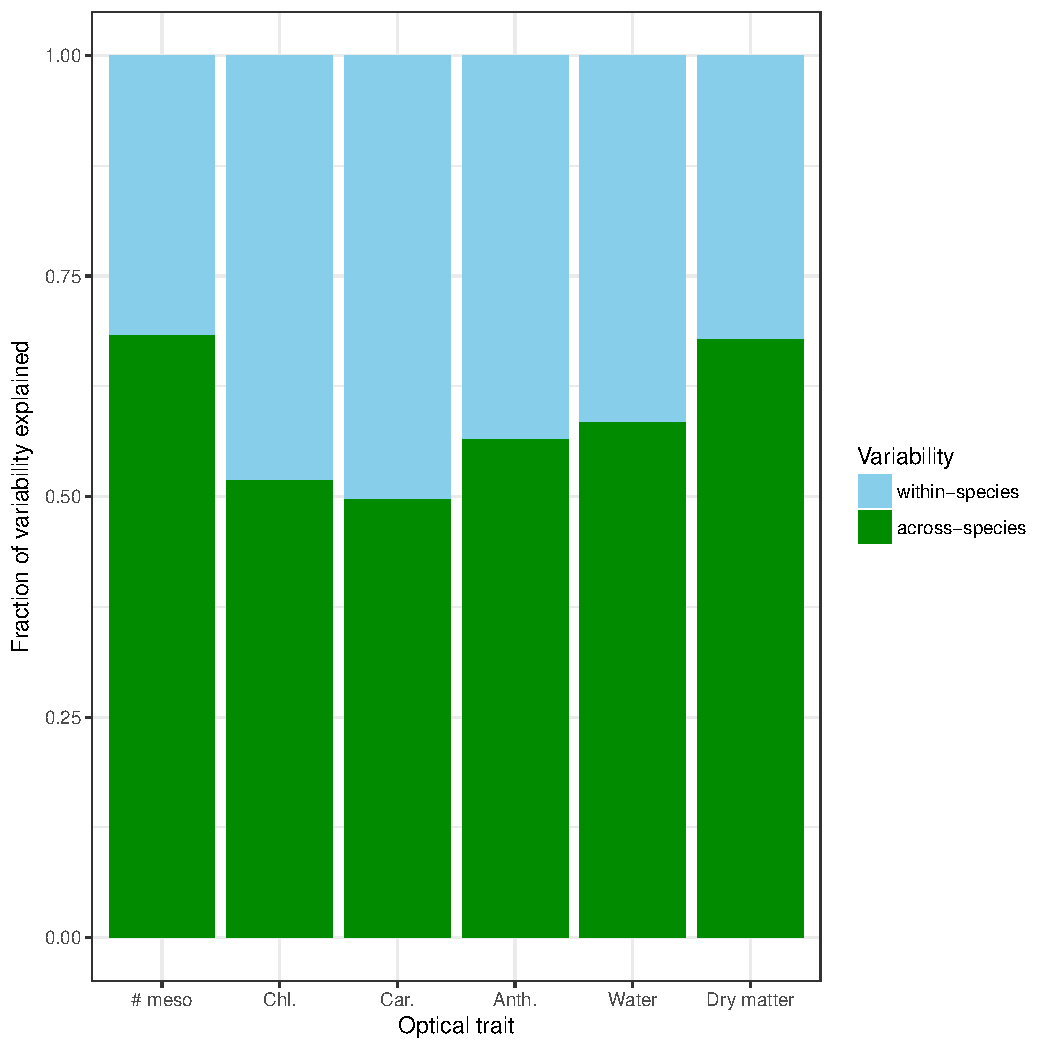
\includegraphics[width=\textwidth]{{figures/within_vs_across}.pdf}
  \caption{\
    Fraction of variance in each optical trait explained by species identity,
    based on analysis of variance on least-squares linear regression.
  }\label{fig:within_vs_across}
\end{figure}

\begin{figure}
  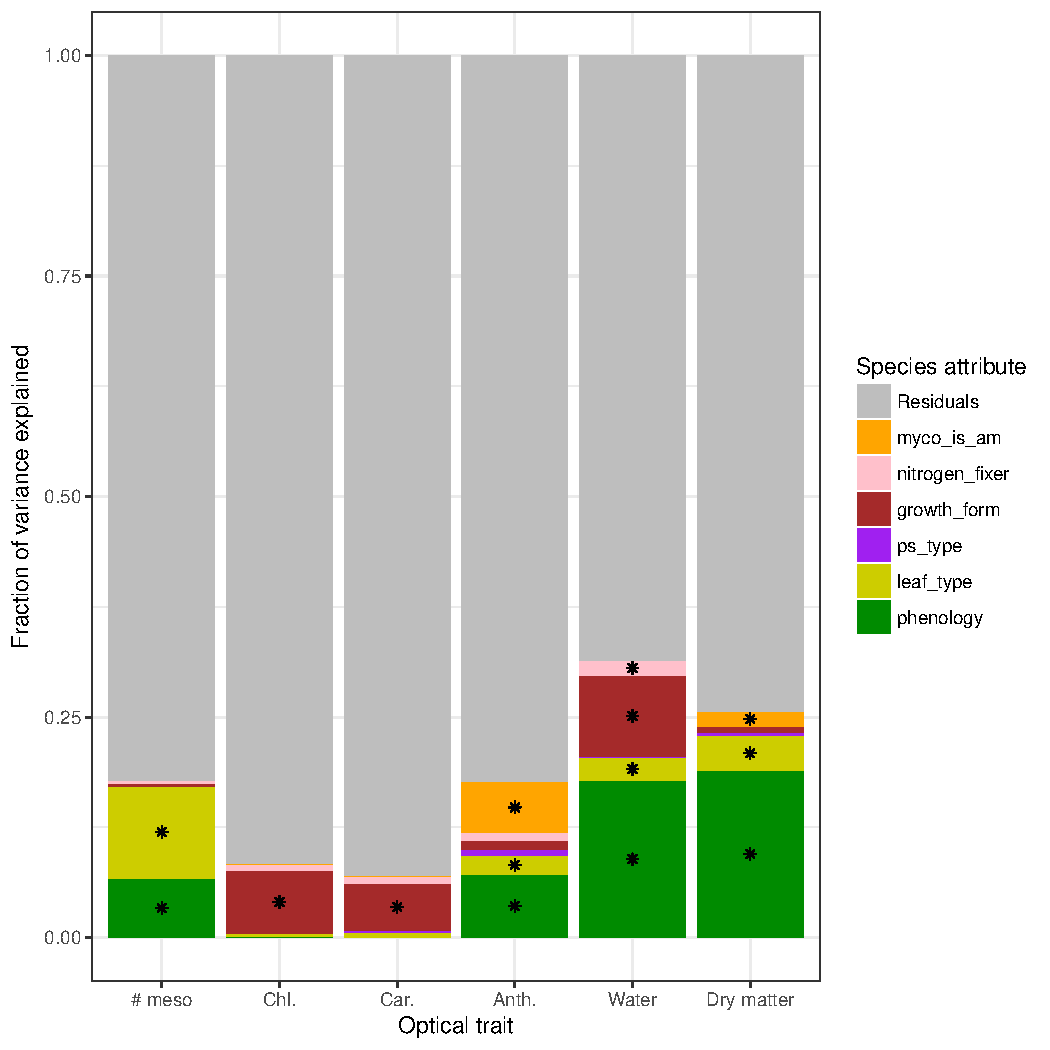
\includegraphics[width=\textwidth]{{figures/across_species_anova}.pdf}
  \caption{\
    Fraction of across-species variance in each optical trait (i.e.~species means) explained by species attributes,
    based on analysis of variance on least-squares linear regression.
    A star (*) indicates attribute effects significant at the 90\% confidence interval.
    Attributes are as follows:
    \texttt{myco\_is\_am} --- Mycorrhizal fungi association (arbuscular or other such as ectomycorrhizal or ericoid);
    \texttt{nitrogen\_fixer} --- whether the species is a Nitrogen fixer;
    \texttt{growth\_form} --- tree, shrub, herb, or grass;
    \texttt{ps\_type} --- photosynthetic pathway (C3 or C4);
    \texttt{leaf\_type} --- leaf morphology (broadleaved or needleleaved);
    \texttt{phenology} --- whether the species is deciduous or evergreen.
  }\label{fig:across_species_anova}
\end{figure}

Across all optical traits, roughly half of variability was explained by species identity (Figure~\ref{fig:within_vs_across}).
The variance across species means was largely idiosyncratic to species, with only up to 25\% of variance explainable by species attributes (Figure~\ref{fig:across_species_anova}).
The most important explanatory attribute was leaf phenology (deciduous vs.~evergreen), with occasional significant effects for leaf type (broad vs.~needle), growth form (woody vs.~herbaceous), and mycorrhizal association (arbuscular or non-arbuscular). 

\begin{figure}
  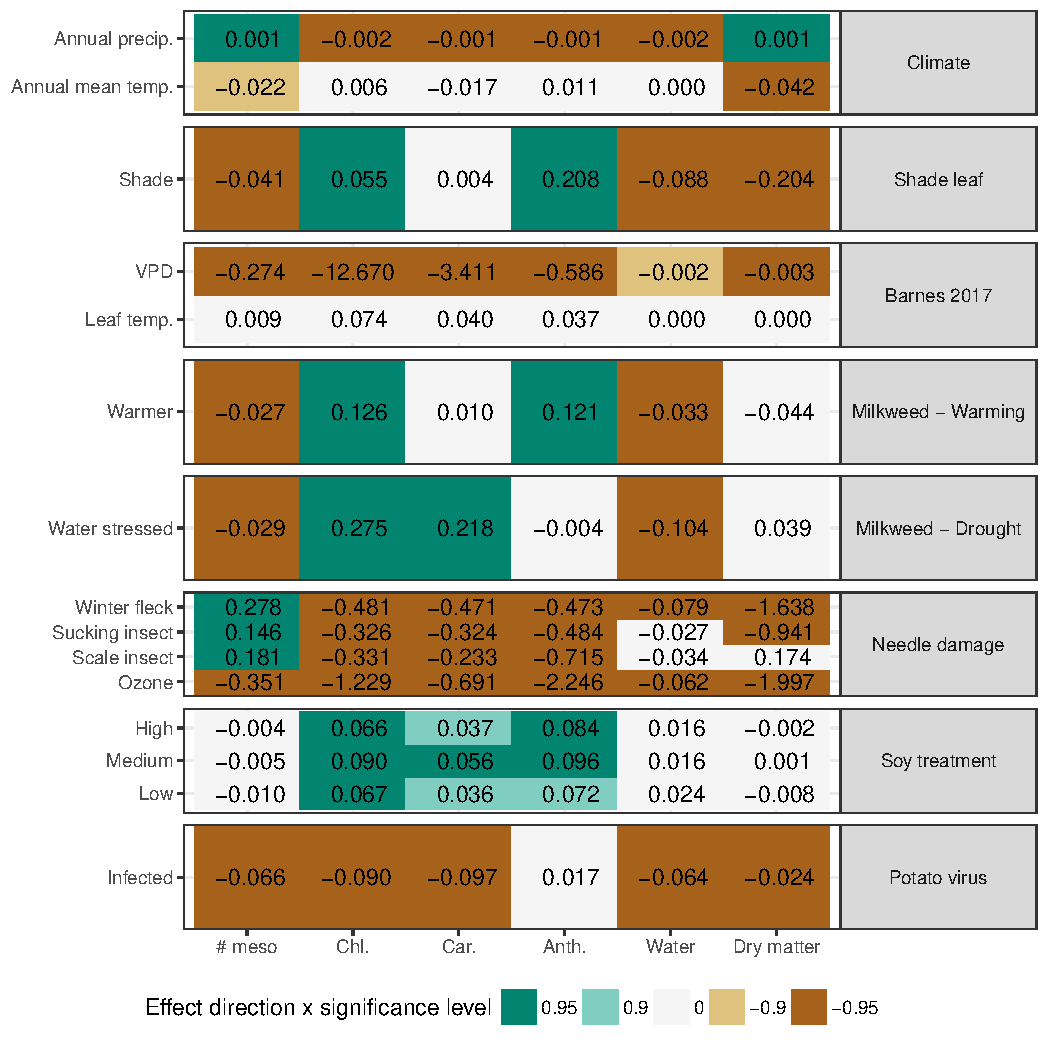
\includegraphics[width=\textwidth]{{figures/treatment_summary}.pdf}
  \caption{\
    Effects of different sources of intraspecific variability on traits estimated via PROSPECT inversion.
    Each value is the fixed effect slope on the corresponding trait normalized to zero mean and unit variance, as estimated from a linear fixed-effects model.
    Color brightness indicates degree of statistical significance (90 or 95\% confidence level), and color hues indicate effect direction (positive or negative).
  }\label{fig:treatment_summary}
\end{figure}

Leaf optical traits responded significantly to a range of natural and experimental stressors (Figure~\ref{fig:treatment_summary}).
Across the entire dataset, intraspecific variability in optical traits was weakly but, in some cases, significantly related to climate, with the strongest effects being declines in mesophyll structure and dry matter content with increasing temperature.
Canopy light environment (i.e.\ whether a leaf was sunlit or shaded) also had a significant effect on most traits, at least for species on which a comparison was possible.
Specifically, shaded leaves showed higher chlorophyll and anthocyanin concentrations and reduced mesophyll structure and water and dry matter contents.

Based on leaf reflectance measurements of \textit{Populus deltoides} (eastern cottonwood) at the University of Arizona by Barnes et al.~(2017), \nocite{barnes_2017_beyond}
seasonal variations in vapor pressure deficit---but not leaf temperature---had significant negative effects on all traits, with the strongest effects on chlorophyll and anthocyanin contents.
Similarly, warming and drought experiments on \textit{Asclepias syriaca} (common milkweed)  had strong and significant effects on almost all optical traits, with both treatments leading to significant decreases in leaf water content and effective number of mesophyll layers and increases in pigments and dry matter content concentrations~\cite{milkweed_data}.
Leaf optical traits also responded significantly to chemical and biotic stressors.
Based on data from Di Vittorio (2009) \nocite{divittorio_2009_enhancing}, needles of \textit{Pinus ponderosa} and \textit{Pinus jeffreyi} from the northern Sierra Nevada mountains experienced reductions in all traits, but most strongly in pigment and dry matter contents,
when afflicted with winter fleck (patchy mortality of needle epidermal cells, usually triggered by exposure to harsh winter weather), sucking and scale insect, and especially ozone damage.
As well, spectral inversion revealed small but statistically significant declines across all optical traits except anthocyanins in \textit{Solanum tuberosum} (potato) plants infected with potato virus Y~\cite{solanum_pvy_data}.
On the other hand, treatment of \textit{Glycine max} (soybean) with aphids resulted in a small but significant increase in pigment concentrations, with the strongest effect observed at medium-level treatment~\cite{soybean_data}.

\begin{figure}
  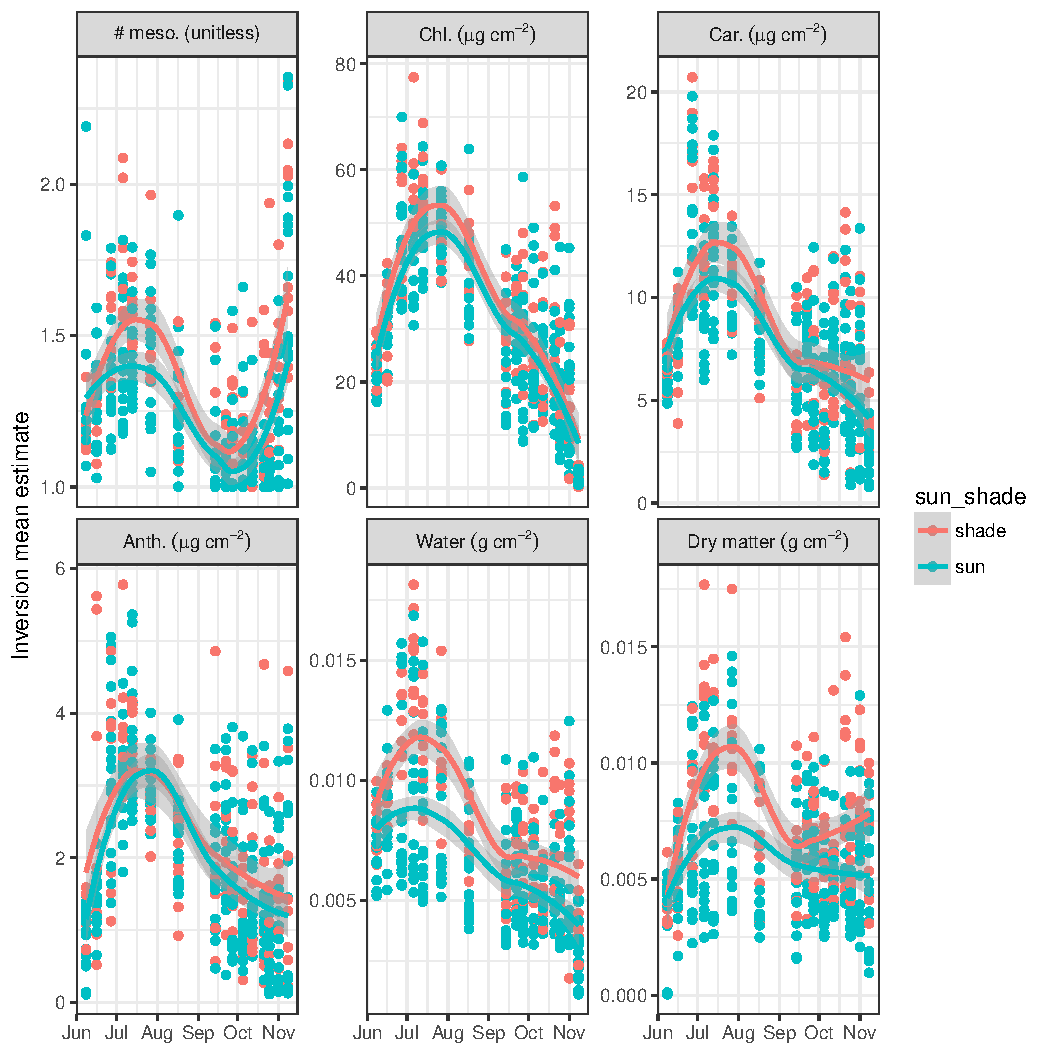
\includegraphics[width=\textwidth]{{figures/trait_phenology}.pdf}
  \caption{\
    Optical trait estimates through a season for \textit{Quercus rubra} (red oak) at Martha's Vineyard, MA by Yang et al.~(2016).
    Colors indicate sunlit vs.~shaded leaves.
    Line is a LOESS best fit with shaded standard error.
  }\label{fig:trait_phenology}
  \nocite{yang_2016_seasonal}
\end{figure}

Where such measurements were available, leaf optical traits exhibited a strong phenological signal (Figure~\ref{fig:trait_phenology}).
All optical traits showed a peak in late July / early August, followed by a decline into the fall, with the sharpest declines for pigments and water content and less precipitous declines for dry matter and mesophyll structure.
Furthermore, the effective number of leaf mesophyll layers, and to a lesser extent, leaf dry matter content in shade leaves, appeared to increase in the late fall.
With the exception of anthocyanin content, all traits for shaded leaves were higher and experienced a greater seasonal variability than sunlit leaves.

\subsection{Trait correlations}

\begin{figure}
  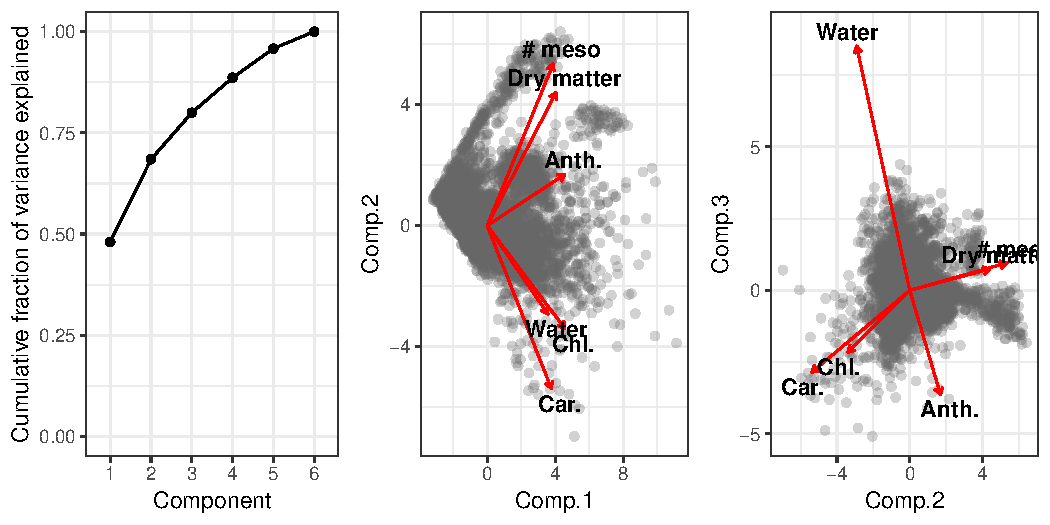
\includegraphics[width=\textwidth]{figures/prospect_pca.pdf}
  \caption{\
    Principal components analysis of optical trait correlation matrix. 
    (Left) Cumulative fraction of variance explained by each principal component.
    (Center, Right) Principal component scores and vectors for each optical trait for components 1 and 2 (center) and 2 and 3 (right).
  }\label{fig:prospect_pca}
\end{figure}

Optical traits estimated by PROSPECT are not mutually independent, but rather have some structure to their covariance (Figure~\ref{fig:prospect_pca}).
In the first two principal components, which collectively explain roughly 70\% of the variability, variation occurs along one of three axes---one defined by chlorophyll, carotenoid, and water contents, another defined by leaf structure and dry matter content, and a third defined by anthocyanin concentration.
% * <dietze@bu.edu> 2018-04-11T13:32:28.770Z:
% 
% > three axes
% Confusing -- how do the first two PCA have 3 axes?
% 
% ^ <emcowdery@gmail.com> 2018-04-12T06:37:57.092Z:
% 
% Three groupings that appear to fall along distinct axes?
% 
% ^.
Variation along the third principal component, which brings the cumulative variance up to roughly 80\%, is defined by a trade-off between water and anthocyanins.

\begin{figure}
  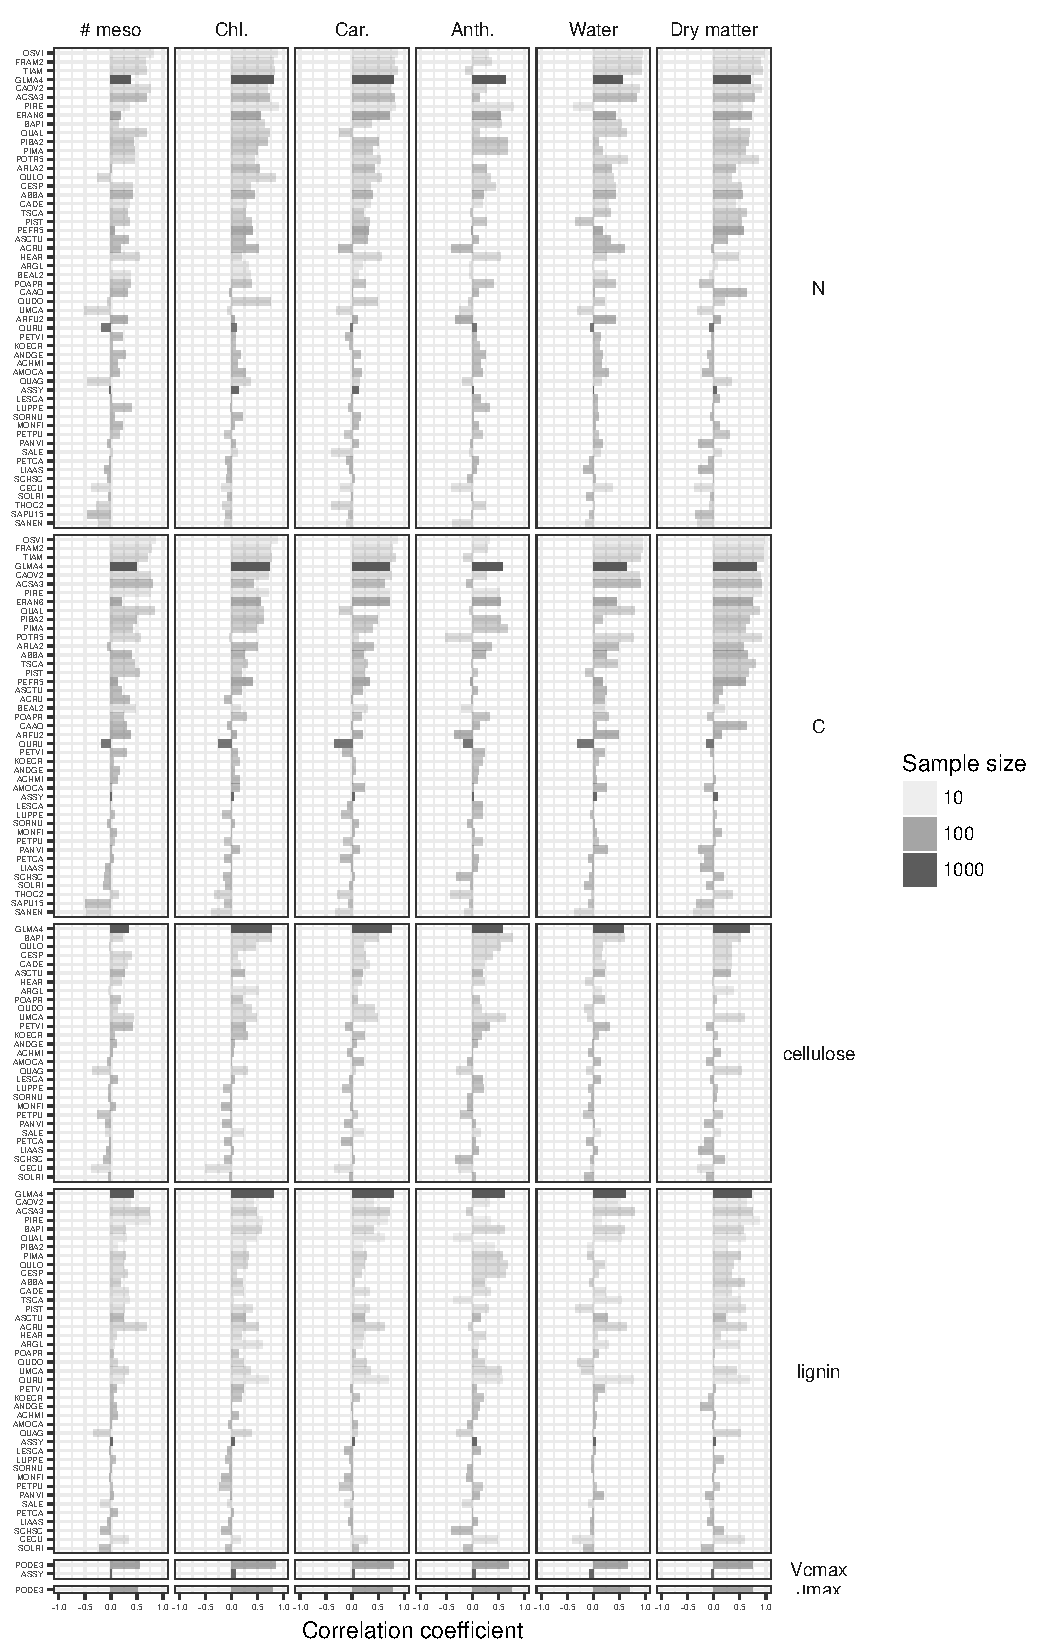
\includegraphics[width=\textwidth]{figures/trait_correlations_areabars.pdf}
  \caption{\
    Intra-specific pairwise correlations of optical traits with direct measurements of
    leaf N, C, cellulose, lignin, Vcmax, and Jmax.
    Darker colors indicate larger sample sizes.
    Species are displayed along the y axis, and are sorted within each facet from highest to lowest average correlation across all traits.
    Analysis was performed only for species with at least 10 pairwise observations of each trait.
% * <dietze@bu.edu> 2018-04-11T14:16:31.779Z:
% 
% Y-axis needs to be explained. Try to make this bigger so the font size isn't so small -- maybe put C and N on one page, and everything else on the next?
% 
% ^.
  }\label{fig:trait_correlations}
\end{figure}

Covariance of optical traits with six area-normalized traits---leaf nitrogen, carbon, cellulose, and lignin contents, Vcmax, and Jmax---was strongly species specific, but, in many cases, substantial (Figure~\ref{fig:trait_correlations}).
% * <dietze@bu.edu> 2018-04-11T14:13:48.873Z:
% 
% > strongly species specific
% 
% Did you not also look at the interspecific correlations? Everything below seems to be intraspecific.
% 
% ^.
In general, for any given species, most of the estimated optical traits exhibited similar correlations with the directly measured trait.
For instance, for soybean (GLMA4), all optical traits were positively correlated with leaf N, C, cellulose, and lignin, whereas for milkweed, all of these correlations were negligible.
Leaf nitrogen correlated best for the largest number of species with leaf chlorophyll and, to a slightly lesser extent, with dry matter content.
Leaf carbon and lignin were most consistently correlated with leaf dry matter content, while correlations with cellulose were more idiosyncratic.
Vcmax and Jmax were strongly positively correlated with all traits for \textit{Populus deltoides} (PODE3), but completely uncorrelated for milkweed (ASSY).

% TODO: Mass traits?

%On a mass basis, leaf number of mesophyll layers and dry matter contents were negatively correlated with direct pigment measurements and protein contents and weakly positively correlated with cellulose, hydrogen, fat, and non-structural carbohydrates.
%Pigments exhibited strong
